
\section{Experiments}
For all experiments, we tune learning rates for the full-horizon un-truncated estimator via grid search over all ${a \times 10^b}$, for ${a \in \{1.0, 2.2, 5.5\}}$ and ${b \in \{0.0, 1.0, 2.0, 3.0, 5.0\}}$.
The same learning rates are used for the truncated estimators and (as reference learning rates) for the RT estimators.
For simplicity, we do not decay the learning rate in any experiments.

We use the same hyperparameters for our online tuning procedure for all experiments: the tuning frequency $K$ is set to $5$, and the exponential moving average weight $\alpha$ is set to $0.9$.
These hyperparameters were not extensively tuned.
For each problem, we compare deterministic truncations with RT-SS and RT-RR estimators, each with different truncations.

\subsection{Lotka-Volterra ODE}
We first experiment with variational inference of parameters of a Lotka-Volterra (LV) ODE. LV ODEs are defined by the predator-prey equations:
\vspace{-1.5\baselineskip}

\begin{align*}
\frac{du_1}{dt} &= A u_1 - B u_1 u_2 &
\frac{du_2}{dt} &= C u_1 u_2 - D u_2
\end{align*}
\vspace{-1.5\baselineskip}

$u_2$ is the predator population, and $u_1$ is the prey population.

We aim to infer the parameters $\lambda = [u_1(t=0), u_2(t=0), A, B, C, D]$.
The true parameters are drawn from $\mathcal{U}([1.0, 0.4, 0.8, 0.4, 1.5, 0.4], [1.5, 0.6, 1.2, 0.6, 2.0, 0.6])$, chosen empirically to ensure stability solving the equations.
We generate ground-truth data by solving the equations using RK4 (a common 4th-order Runge Kutta method) from $t = 0$ to $t = 5$ with $10000$ steps.
The learner is given access to five equally spaced noisy observations $y(t)$, generated according to $y(t) = u(t) + \mathcal{N}(0, 0.1)$.

We place a diagonal Gaussian prior on $\theta$ with the same mean and standard deviation as the data-generating distribution.
The variational posterior is a diagonal Gaussian $q(\lambda)$ with mean $\mu$ and standard deviation $\sigma$.
The parameters optimized are $\theta = [\tilde{\mu}, \tilde{\sigma}]$.
We let $\mu = g(\tilde{\mu})$ and $\sigma = g(\tilde{\sigma})$, where $g(x) = \log(1+e^{\tilde{x}})$, to ensure positivity.
We use a reflecting boundary to ensure positivity of parameter samples from $q$.
The variational posterior is initialized to have mean equal to the prior and standard deviation 0.1.

The loss considered is the negative evidence lower bound (negative ELBO). The ELBO is:
\begin{align*}
\text{ELBO}(q(\theta))\!&=\! \mathbb{E}_{q(\theta)}\! \sum_{t}\! \log p(y(t) | u_\theta(t))\! +\! D_{\sf{KL}}\big(q(\theta) || p(\theta) \big)
\end{align*}
Above, $u_\theta(t)$ is the value of the solution $u_\theta$ to the LV ODE with parameters $\theta$, evaluated at time $t$.
We consider a sequence $\mathcal{L}_n(\theta)$, where in computing the ELBO, $u_\theta(t)$ is approximated by solving the ODE using RK4 with $2^n + 1$ steps,
and linearly interpolating the solution to the $5$ observation times.
The outer-loop optimization is performed with a batch size of $64$ (i.e., $64$ samples of $\theta$ are performed at each step) and a learning rate of $0.01$.
Evaluation is performed with a batch size of $512$.

\begin{figure}
\vspace{-0.3cm}
\small
\begin{tabular}{c c}
\rotatebox{90}{\qquad\qquad$\text{Negative ELBO}$}&
\hspace{-2mm}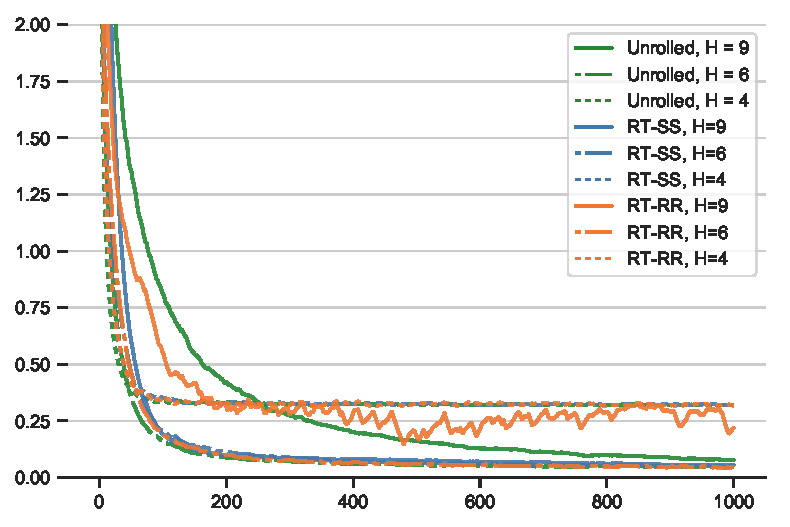
\includegraphics[width=0.9\linewidth, clip, trim=2mm 2mm 0cm 0cm]{rt/plots/lv_sgd_new/test_horizon_loss.pdf} \vspace{-1mm} \\
& \vspace{-2mm} Gradient evaluations (000s)
\label{fig:lv_loss}
\end{tabular}
\caption{Lotka-Volterra parameter inference}
\vspace{-0.5cm}
\end{figure}

Figure \ref{fig:lv_loss} shows the loss of the different estimators over the course of training.
RT-SS estimators outperform the un-truncated estimator without inducing bias.
They are competitive with the truncation~${H = 6}$, while avoiding the bias present with the truncation~${H = 4}$.
By contrast, some RT-RR estimators experience issues with optimization, falling into the same local minimum as the $H = 4$ truncation.

\subsection{MNIST learning rate}
We next experiment with meta-optimization of a learning rate on MNIST.
We largely follow the procedure used by \cite{wu2018understanding}.
We use a feedforward network with two hidden layers of 100 units, with weights initialized from a Gaussian with standard deviation 0.1, and biases initialized to zero.
Optimization is performed with a batch size of 100.

The neural network is trained by SGD with momentum using Polyak averaging, with the momentum parameter fixed to $0.9$.
We aim to learn a learning rate $\eta_0$ and decay $\lambda$ for the inner-loop optimization.
These are initialized to $0.01$ and $0.1$ respectively.
The learning rate for the inner optimization at an inner optimization step $t$ is~$
{\eta_t = \eta_0(1 + \frac{t}{5000})^{-\lambda}}$.

As in \cite{wu2018understanding}, we pretrain the net for 50 steps with a learning rate of $0.1$.
$\mathcal{L}_n$ is the evaluation loss after $2^n + 1$ training steps with a batch size of $100$.
The evaluation loss is measured over $2^n + 1$ validation batches or the entire validation set, whichever is smaller.
The outer optimization is performed with a learning rate of $0.01$.

RT estimators with $H = 9$ or $H = 5$ achieve faster convergence than the fixed-truncation estimators.
RT-SS outperforms RT-RR.
All estimators with $H = 5$ appear to suffer from some bias.
The un-truncated estimator achieves a slightly better loss than the RT estimators, but takes significantly longer to converge.

\begin{figure}
\vspace{-0.3cm}
\small
\begin{tabular}{c c}
\rotatebox{90}{\qquad\qquad$\text{Evaluation loss}$}&
\hspace{-2mm}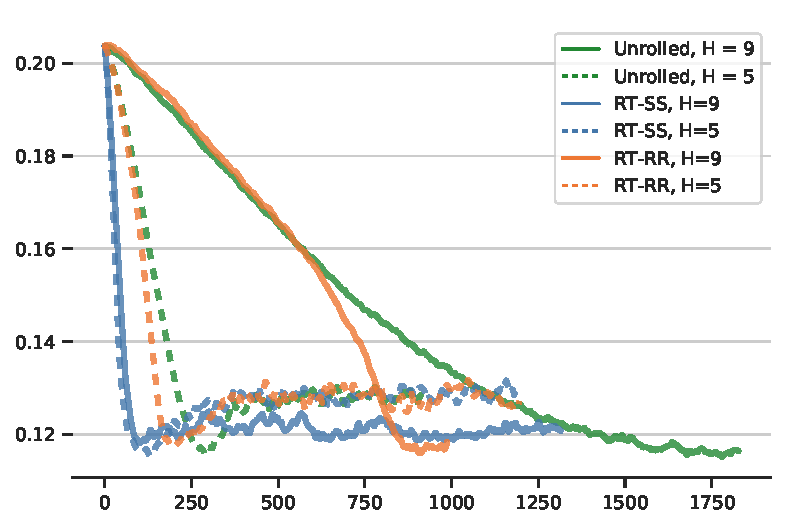
\includegraphics[width=0.9\linewidth, clip, trim=2mm 2mm 0cm 0cm]{rt/plots/mnist_sgd/fullhorizon_eval_cross_entropy.pdf} \vspace{-1mm} \\
& \vspace{-2mm} Neural network evaluations (000s)
\label{fig:mnist_loss}
\end{tabular}
\caption{MNIST learning rate meta-optimization}
\vspace{-0.1cm}
\end{figure}

\subsection{\texttt{enwik8} LSTM}
Finally, we study a high-dimensional optimization problem:
training an LSTM to model sequences on $\texttt{enwik8}$.
These data are the first 100M bytes of a Wikipedia XML dump.
There are 205 unique tokens. We use the first 90M,
5M, and 5M characters as the training, evaluation, and test sets.

We build on code from
\cite{merity2017regularizing, merity2018analysis} found at
https://github.com/salesforce/awd-lstm-lm. We train
an LSTM with 1000 hidden units and 400-dimensional input and output
embeddings. The model has 5.9M parameters. The only regularization is
an $\ell_2$ penalty on the weights with magnitude $10^{-6}$.
Gradients are clipped to magnitude $1.0$ before each optimization step.
The optimization is performed with a learning rate of $2.2$.
This model is not state-of-the-art: our aim to investigate performance of
RT estimators for optimizing high-dimensional neural networks, rather than to
maximize performance at a language modeling task.

We choose $\mathcal{L}_n$ to be the mean
cross-entropy after unrolling the LSTM training for $6 * 2^n + 1$ steps.
We choose the horizon $H = 5$, such that
the un-truncated loop has 193 steps, chosen to be approximately equal to the
200-length training sequences used by \cite{merity2018analysis}.

Figure \ref{fig:enwik} shows the training bits-per-character (proportional to the training cross-entropy loss).
All RT estimators provide some acceleration over the un-truncated~${H=5}$ estimator early in training.
RT-SS underperforms relative to RT-RR.
Within the first 100k cell evaluations, the RT estimators fall back on the un-truncated estimator,
subsequently progressing slightly more slowly due to computational cost of tuning.
We conjecture that the covariance assumptions in Section 5 are often unsuited to high-dimensional problems, and lead to overly conservative estimators.

\begin{figure}
\vspace{-0.3cm}
\small
\begin{tabular}{c c}
\rotatebox{90}{\qquad$\text{Training bits-per-character}$}&
\hspace{-2mm}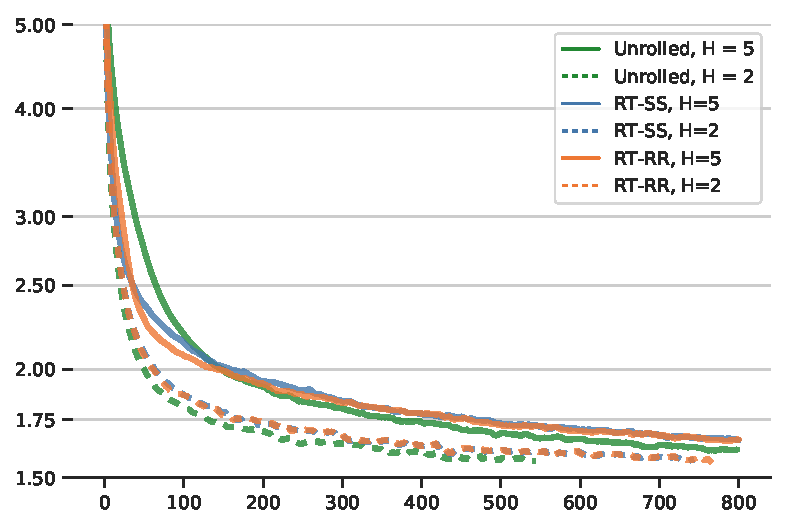
\includegraphics[width=0.9\linewidth, clip, trim=2mm 2mm 0cm 0cm]
{rt/plots/enwik_sgd/train_bpc.pdf} \vspace{-1mm} \\
& \vspace{-2mm} LSTM cell evaluations (000s)
\label{fig:enwik}
\end{tabular}
\caption{LSTM training on \texttt{enwik8}}
\vspace{-0.1cm}
\end{figure}
